\documentclass[svgnames,11pt]{standalone}
\usepackage[utf8]{inputenc}
\usepackage[T1]{fontenc}
\usepackage[english]{babel}
\usepackage{amsmath,amssymb}
\usepackage{enumitem}
\usepackage{graphicx}
\usepackage{microtype}
\usepackage{multicol}
\usepackage{tikz}
\usepackage{times}
\usepackage{xcolor}
\usetikzlibrary{arrows,automata}
\newcommand{\poslabel}{$1$}
\newcommand{\neglabel}{$0$}
\newcommand{\epslabel}{}
\newcommand{\minuslabel}{$-1$}
\begin{document}

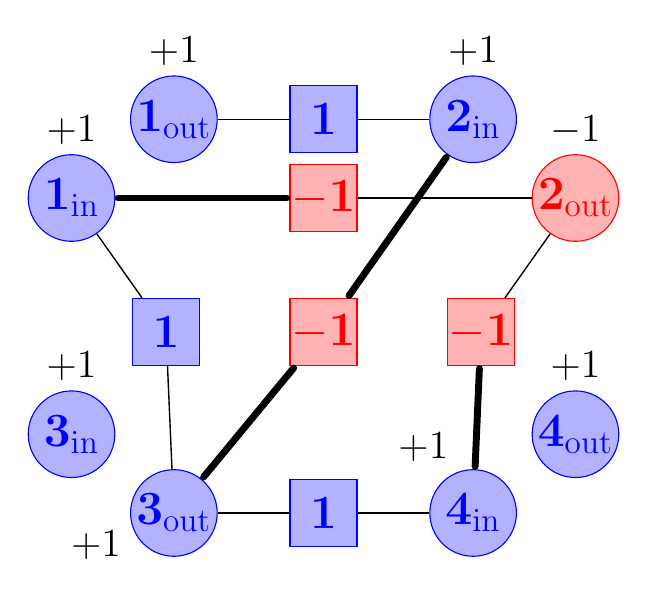
\begin{tikzpicture}[auto, every label/.style={font=\Large}]
\tikzset{>=latex}
\tikzstyle{peers}=[draw,circle,black,minimum width=11mm,inner sep=0]
\tikzstyle{nedge}=[draw,rectangle,black,minimum width=8.5mm,minimum height=8.5mm, inner sep=0]
\tikzstyle{edge}=[line width=0.5pt,color=Black,->]
\tikzstyle{uedge}=[line width=0.5pt,color=Black]
\tikzstyle{phi}=[line width=2.5pt,line cap=round,shorten <= 1pt, shorten >= 1pt]
\tikzstyle{pnode}=[fill=White]
\tikzstyle{elabel}=[color=Black]
\tikzstyle{qnode}=[fill=White]
% \tikzstyle{posc}=[color=blue]
% \tikzstyle{negc}=[color=red]


\tikzstyle{posc}=[color=blue, fill=blue!30!white]
\tikzstyle{negc}=[color=red, fill=red!30!white]
\node[peers,pnode,posc,label={$+1$}] (p1) at (1.3, -1.0) {\LARGE$\mathbf{1_{\mathrm{out}}}$}; 
\node[peers,pnode,negc,label={$-1$}] (p2) at (6.4, -2.0) {\LARGE$\mathbf{2_{\mathrm{out}}}$}; 
\node[peers,pnode,posc,label=190:{$+1$}] (p3) at (1.3, -6.0) {\LARGE$\mathbf{3_{\mathrm{out}}}$}; 
\node[peers,pnode,posc,label={$+1$}] (p4) at (6.4, -5.0) {\LARGE$\mathbf{4_{\mathrm{out}}}$}; 
\node[peers,qnode,posc,label={$+1$}] (q1) at (0.0, -2.0) {\LARGE$\mathbf{1_{\mathrm{in}}}$}; 
\node[peers,qnode,posc,label={$+1$}] (q2) at (5.1, -1.0) {\LARGE$\mathbf{2_{\mathrm{in}}}$}; 
\node[peers,qnode,posc,label={$+1$}] (q3) at (0.0, -5.0) {\LARGE$\mathbf{3_{\mathrm{in}}}$}; 
\node[peers,qnode,posc,label=110:$+1$] (q4) at (5.1, -6.0) {\LARGE$\mathbf{4_{\mathrm{in}}}$}; 
 \node[nedge,posc] (e1) at (3.2, -1.0) {\LARGE$\mathbf{1}$}; 
 \node[nedge,negc] (e2) at (3.2, -2.0) {\LARGE$\mathbf{-1}$}; 
 \node[nedge,negc] (e3) at (5.2, -3.7) {\LARGE$\mathbf{-1}$}; 
 \node[nedge,posc] (e4) at (1.2, -3.7) {\LARGE$\mathbf{1}$}; 
 \node[nedge,negc] (e5) at (3.2, -3.7) {\LARGE$\mathbf{-1}$}; 
 \node[nedge,posc] (e6) at (3.2, -6.0) {\LARGE$\mathbf{1}$};



\draw[uedge] (p1) edge [bend left=0] node [elabel,below] {\epslabel} (e1);
\draw[uedge] (e1) edge [bend left=0] node [elabel,below] {\epslabel} (q2);
\draw[uedge] (p2) edge [bend left=0] node [elabel,above,yshift=-1mm,pos=.25] {\epslabel} (e2);
\draw[uedge,phi] (e2) edge [bend left=0] node [elabel,above,yshift=-1mm] {\epslabel} (q1);
\draw[uedge] (p2) edge [bend left=0] node [elabel] {\epslabel} (e3);
\draw[uedge,phi] (e3) edge [bend left=0] node [elabel] {\epslabel} (q4);
\draw[uedge] (p3) edge [bend left=0] node [elabel] {\epslabel} (e4);
\draw[uedge] (e4) edge [bend left=0] node [elabel,above,xshift=1mm,pos=.35] {\epslabel} (q1);
\draw[uedge,phi] (p3) edge [bend left=0] node [elabel,above,xshift=-1mm] {\epslabel} (e5);
\draw[uedge,phi] (e5) edge [bend left=0] node [elabel,below,xshift=1mm,pos=0.3] {\epslabel} (q2);
\draw[uedge] (p3) edge [bend left=0] node [elabel] {\epslabel} (e6);
\draw[uedge] (e6) edge [bend left=0] node [elabel] {\epslabel} (q4);

\end{tikzpicture}
\end{document}
